\subsection{溶液的物理性质}
如上所述,溶解度和过饱和度有时可通过一些物理参数来间接测定,晶体生长中有许多关系式也涉及到一些溶液的物理性质。在本节中将对其中一些性质作简要叙述。

\paragraph{(1) 密度}
溶液的浓度常用密度来表示。密度定义为单位体积的质量:$\rho=m/V \ {\rm (kg\cdot m^{-3})}$。

在某一温度下,液体的密度和水的密度之比称为液体的比重。 因密度是受温度影响的,因此比重数据需标明温度。例如溶液比重为1.23(20/20℃),即表示在20℃时,溶液的密度和水的密度之比(不标明时,均指20℃),而1.23(20/4℃)则指20℃时的溶液密度和4℃时水的密度的比值。4℃时水的密度具有最大值${\rm kg\cdot m^{-3}}$,因此溶液与4℃时的水相比之比重在数值上等于在给定温度下的密度。

测量密度的方法有多种,其中最方便的方法是用比重计。 
一些常用的溶剂比重见表3.3。

\paragraph{(2) 粘度}
粘度是流体对于流动所表现出的阻力的量度,即流体的内摩擦。溶液的粘度对结晶过程(成核,晶体生长)、热量和质量的传输过程等影响都很显著。

粘度$\eta$(粘度系数或绝对粘度)定义为在流体内部单位面积内单位速度梯度的切应力。其单位为$\rm Pa\cdot s = kg\cdot m^{-1}\cdot s^{-1}$。

液体的粘度随温度升高而减少。对多数液体来既,存在以下的关系式:
\begin{equation}
\eta = A\exp{(-B/T)},
\end{equation}
$A$,$B$为常数,$T$为绝对温度。以$\log{\eta}$对$1/T$作图,所得的图形为直线。表3.4列出了一些普通溶剂在一定温度范围内的粘度数值。

%TODO:表3.4
(表3.4)

\paragraph{(3) 扩散率(扩散系数)}
扩散对于结晶和溶解过程都是十分重要的。在生长晶体的过程中,结晶物质(溶质)通过体扩散和 溶剂分子运动输送到晶体附近,通过扩散层到晶体表面,再借助于面扩散进入生长位置。扩散系数定义为在单位浓度梯度下,每单位时间内通过单位面积的质点的数目(或摩尔数),在实验上要准确测定扩散系数是比较困难的。

爱因斯坦基于动力学理论和关于粒子在液体中运动的斯托克斯(Stockes)定律,得出关于扩散系数的表达式为
\begin{equation}
D=\frac{kT}{\phi r\eta},
\end{equation}
式中$D$为扩散系数($\rm m^2\cdot s^{-1}$),$T$为绝对温度,$\eta$为液体的粘度($\rm Pa\cdot s$),$r$为质点的半径,$k$为玻尔兹曼常量,因子$\phi$的数值在$4\pi$到$6\pi$之间(取决于溶质和溶剂分子大小的比值)。由于在式(3.12)中含有很难测定的溶质分子半径$r$,更为直接有用的关系式为
\begin{equation}
\frac{D\eta}{T}=\text{常数},
\end{equation}
这一简单关系式称为斯托克斯—爱因斯坦方程。根据式(3.13)就可以预测温度和粘度对扩散系数的影响。

爱因斯坦还研究了位移布朗运动的理论,得出以下关系式:
\begin{equation}
x^2=2Dt
\end{equation}
$x$为扩散质点在$t$时间内的平均位移,$D$是扩散系数,将式(3.12)代入上式,并取$\phi=6\pi$,则可得
\begin{equation}
x^2=2Dt=\frac{kTt}{3\pi\eta r}
\end{equation}
这就是爱因斯坦—布朗运动公式。该式很容易用实验来验证,并在研究晶体生长的表面扩散过程中起着很重要的作用。

\paragraph{(4) 折射率}
通过测量溶液的折射率,可迅速确定溶液的浓度。常用的测量装置是阿贝折射仪。对于研究结晶过程,读数精确到小数第四位就足够了。考虑到温度的影响,在进行实际测量前,还需作校正曲线。如使用浸没式折射仪,还可对溶液结晶时的浓度变化进行半连续的测量。由于结晶时溶液中有大量微晶散射光线,使稜镜得不到充分的照明,为此可利用光纤从外部对稜镜\footnote{编者注:原文如此。}周围进行照明。图3.13示出用阿贝折射仪在40℃时测定的KDP、DKDP和ADP的折光指数与溶液浓度的关系。

%图3.13

\begin{figure}[htb]
 \centering
 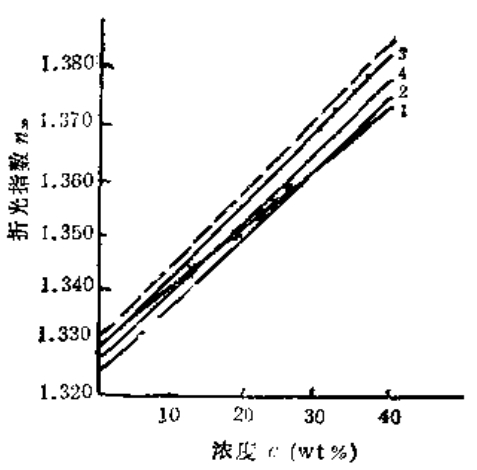
\includegraphics[width=0.4\textwidth]{fig/cp03/img3.13.jpg}
 \caption{几种溶液的折光指数对浓度曲线。}
 $t_{\rm K_4}, t_{\rm DK_4},t_{\rm A_4}$分别表示温度为40℃的KDP,DKDP和ADP溶液。
 
 $t_{\rm DK_2}$示温度为20℃的DKDP溶液。实线是激光,虚线为钠光。
\end{figure}

\paragraph{(5) 电导率}
水溶液的电导率可以十分精确地测量出来,因此可作为测量浓度的有效方法。但已做的工作大都局限于稀溶液体系,在接近饱和和过饱和溶液中所得到的测量结果常不可靠。由于电导率也和温度有关,所以要求有高精度的控温。

\paragraph{(6) 热导率}
物质的热导率$\kappa$定义为在单位温梯度下,横过垂直于热传导方向的单位面积,经过单位厚度层的热传导速度。 恒稳状态的热传导方程可以写成
\begin{equation}
dQ/dt=-\kappa A\frac{dT}{dx},
\end{equation}
式中$Q,t,A,T$和$x$分别代表热量、时间、面积、温度和厚度的单位。

液体的热率一般随温度的升高而稍有下降,但水是例外。表3.5列出了一些纯液体的热导率。目前尚缺乏测量热导率的可靠方法。在文献中很少报道有关热导率的数据(特别是溶液的热导率),即使有报道也常常是相互矛盾的。

%TODO: 表3.5
(表3.5)

\paragraph{(7) 溶解热和结晶热}
当溶质溶解在溶剂中而不发生反应时,通常从周围环境吸收热量(溶解热),如溶解在绝热条件下进行,则溶液温度将下降。当溶质从溶液中结晶出来时,通常有热量放出(结晶热),溶液温度将上升。但当溶质和溶剂存在化学反应(溶剂合作用)时,对于一些溶解度温度系数为负的溶质来说,也会出现溶解时放热和结晶时吸热现象。无水盐在其水合物为稳定晶形的温度下溶于水中时,由于水合过程的放热特性故有热量放出
$$\rm AB\text{(无水物)} + \mathit{x}H_2O\rightarrow AB\cdot\mathit{x}H_2O\text{(水合物)}.$$
表3.6列出了硫酸镁和碳酸钠的无水物及水合物的溶解热数据,从表中可看出结晶水的效应。

(表3.6)

在一定量溶剂或不饱和溶液中,溶质溶解的热效应的大小取决于溶质和溶剂的数量。溶液的起始和最终浓度以及溶解时的温寞,常用的标准参考温度是25 ℃或18℃。

溶解热和结晶热可分别用在溶解和结晶过程中焓的变化$\Delta H_s$,和$\Delta H_c$来表示。由于用实验直接测量结晶热较为困难,故常常通过溶解热来求。在实用上,常把结晶热和溶解热看成数值相等而符号相反,即
\begin{equation}
\Delta H_c = -\Delta H_s,
\end{equation}
这一假定是不很严格的,但误差不大。溶解热通常是指将单位量(如1mol)的溶质溶解在大量纯溶剂中时焓的变化,即无限稀释时的溶解热$\Delta H^{\infty}_s$(实际上溶质在溶液中的摩尔数小于0.01,即相当于无限稀释),只有当溶质在一定温度下溶于接近饱和的溶液中时,结晶热在数值上才等于溶解热。因此,要求出结晶热的准确数值,还必须考虑稀释热$\Delta H_d$,即
\begin{equation}
\Delta H_c = -\Delta H^{\infty}_s + \Delta H_d.
\end{equation}
由于大多数水溶性盐的溶液在稀释时是放热的(浓缩时吸热),因此结晶热的实际值要比按式(3.16)所计算的值稍低些。

结晶热是重要的物理化学参量,它在研究结晶过程的热平衡和动力学方面有着重要的作用。

